\section{AOTF}

The fundamental piece of technology that allows for the building of ALI is an Acousto-Optical Tunable Filter (AOTF) which allows a signal to be passed through a band gap wavelength filter. The use of AOTF technology for space based initiatives is only recently possible due the recent advances in creating AOTFs with the ability to maintain imaging qualities over a wide acceptance angles. This section will discuss the theory behind the AOTF as well as the calibration and testing of the specific AOTF used for the ALI instrument.

\subsection{Background and Theory}

An AOTF is a device that through phonon-phonon interactions and Bragg diffraction allows a broadband light source to be filtered into a spectral image. Two primary types of AOTF's exists, a collinear (\emph{i.e.} the acoustic wave is collinear with the incident beam, \citep{Harris1969} and a non-collinear (\emph{i.e.} the acoustic wave and the optical beam do not propagate collinearly in the crystal, \citep{Chang1977} configurations and both use an optically anisotropic medium \citep{Saito1976}. An anisotropic medium is a material that is transparent and has a different index of refraction based upon the polarization of the incoming light and its propagation direction, commonly called birefringence. In order to fully understand the principles behind an AOTF two methods shall be used, first a stress analysis through the acousto-wave and a second by the required diffraction momentum matching criteria. A piezo-electric transducer is attached to a face of the anisotropic crystal that allows a Radio Frequency (RF) to be passed into the crystal which affects permittivity. This causes an acoustic wave to be formed within the crystal, essentially forming a pressure wave throughout the entire crystal. If we assume that the pressure wave causes a stress throughout the crystal then a modulation of the permittivity or dielectric constant will occur as,
\begin{equation}
    \ \epsilon = \epsilon_{0} + \epsilon_{1}\cos(\Omega t - \boldsymbol\kappa \boldsymbol\cdot \mathbf{r})
    \label{eqn:3.1:dielectricMod}
\end{equation}
where $\epsilon$ is the new permittivity due to the the pressure wave, $\epsilon_{0}$ is the original permittivity, and $\epsilon_{1}$ is the perturbation component of the permittivity due to the stress wave. The frequency and wave vector of the acoustic wave are $\Omega$ and $\boldsymbol\kappa$ respectively. The primary terms in the acoustic waves are related as follows
\begin{equation}
    \ \frac{\Omega}{\kappa} = \Lambda F = \nu
    \label{eqn:3.1:acoustoWaveDef}
\end{equation}
where $\Lambda$ is the wavelength of the acoustic wave and $F$ is the frequency with $\nu$ being the respective velocity in the birefringent material. Since the permittivity is now a function of time and space an analysis must be done by Maxwell's equations to determine the form of the interacted electric field, $\mathbf{E}$ to determine if a plane wave can still be assumed.

\begin{equation}
    \ \nabla \times \mathbf{E} + \frac{\partial \mathbf{B}}{\partial t} = 0
    \label{eqn:3.1:faradaysLaw}
\end{equation}
\begin{equation}
    \ \nabla \times \mathbf{B} = \mathbf{J} + \frac{\partial(\epsilon \mathbf{E})}{\partial t}
    \label{eqn:3.1:amperesLaw}
\end{equation}

The curl of the \autoref{eqn:3.1:faradaysLaw} and \autoref{eqn:3.1:amperesLaw} can be combined with the fact that the AOTF crystal is non-conductive; therefore $\mathbf{J} = 0$ which gives the simplified form
\begin{equation}
    \ -\nabla^{2} \mathbf{E} + \nabla (\nabla \cdot \mathbf{E}) = -\mu \frac{\partial^{2} (\epsilon \mathbf{E})}{\partial t^{2}}.
    \label{eqn:3.1:electricFieldDE}
\end{equation}
Given that the divergence of the dielectric displacement is zero and the permittivity varies with space, the following relation can be found for the divergence of the electric field.
\begin{equation}
    \ \nabla \cdot \mathbf{E} = -\mathbf{E} \cdot \ln{\epsilon}
    \label{eqn:3.1:divergenceEField}
\end{equation}

The above can be inserted into \autoref{eqn:3.1:electricFieldDE} to give the following relation
\begin{equation}
    \ -\nabla^{2} \mathbf{E} + \nabla (-\mathbf{E} \cdot \ln{\epsilon}) = -\mu \frac{\partial^{2} (\epsilon \mathbf{E})}{\partial t^{2}}.
    \label{eqn:3.1:electricFieldDEAcousticWave}
\end{equation}
However, the simplified divergence term can be shown to be on the order of $\lambda /\Lambda$ which is small and therefore can be neglected leaving the following differential equation:
\begin{equation}
    \ \nabla^{2} \mathbf{E} = \mu \frac{\partial^{2}}{\partial t^{2}}\epsilon \mathbf{E}
    \label{eqn:3.1:eletricFieldAcoustoWave}
\end{equation}

The above differential equation allows for a plane wave to be used for the outgoing light as the interaction does not greatly effect the form of the outbound electric field. A standard acousto-optical experiment is shown in \autoref{fig:3.1:AOTFExperimentalSetUp}. The acoustic wave is propagating in the x direction of the crystal causing the described stress which leads to the modulation of the index of refraction within the acoustic region of the crystal denoted by $L$. The light is incident at an angle $\theta$ with respect to the normal of the crystal surface and the electric field entering the device will be a plane wave described by
\begin{equation}
    \ \mathbf{E}_{i} = \mathbf{E}_{0}\exp[j(\omega t-kx\sin \theta - kz \cos \theta)].
    \label{eqn:3.1:planeWaveEField}
\end{equation}

\begin{figure}
    \begin{center}
    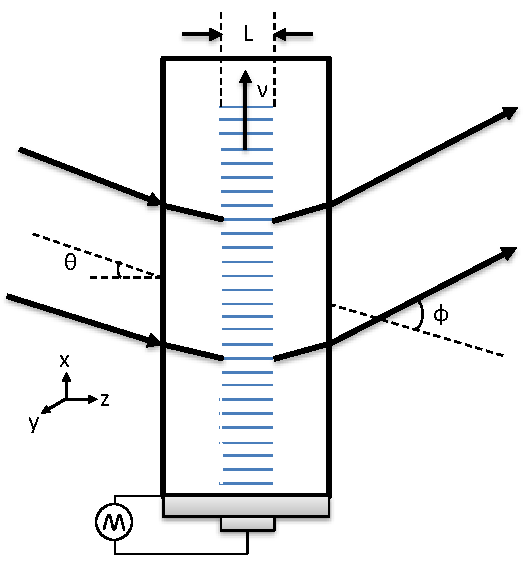
\includegraphics{./Images/3-1-AOTFExperimentSetUp.pdf}
    \caption[AOTF Experimental Set Up]{A standard non-collinear AOTF experiential set up. The crystal is assumed to infinitely long in the y direction. Figure recreated after \cite{Guenther1990} number 14B-1.}
    \label{fig:3.1:AOTFExperimentalSetUp}
    \end{center}
\end{figure}

The incoming electric field is modulated by the acoustic wave propagating through the crystal. Since the acoustic wave is periodic, it can expanded into the following Fourier series of a plane wave though the acoustic interaction, which gives the diffracted electric field $\mathbf{E}_{d}$.
\begin{equation}
    \ \mathbf{E}_{d} = \sum_{i=-\infty}^{\infty}\mathbf{E}_{i}\exp{(j[(\omega+\Omega_{i})t+(\kappa_{i}-k\sin\theta)x-kz\cos\theta]})
    \label{eqn:3.1:modulatedEField}
\end{equation}

It should be noted that the frequency of the $i$th order diffracted light is now Doppler shifted and has become $\omega+\Omega_{i}$, however for an AOTF experiencing Bragg diffraction only the first term of the acousto interaction diffracts causing $\Omega_{1}$ to be small compared to $\omega$ so a negligible shift in the wavelength of the diffracted beam $\mathbf{E}_{d}$ occurs. Bragg Diffraction occurs when the active region of the acoustic wave, $L$, is much larger than the diffracted wavelength, causing the stress wave in the crystal to act as a thick diffraction grating. The above also tells us the x component of the wave vector for the $i$th order is
\begin{equation}
    \ k_{ix} = \kappa_{i}-k\sin\theta = k_{i}\sin\phi_{i}
    \label{eqn:3.1:diffractedWaveVectorXdir}
\end{equation}
where $k_{i}$ is the wave vector of the $i$th order of diffracted beam, the angle $\phi_{i}$ is between the incident beam and the diffracted beam.  The magnitude of the diffracted wave vector is
%For an AOTFs undergoing Bragg diffraction $\theta = \theta_{B}$ where $\theta_{B}$ is the Bragg's angle.
\begin{equation}
    \ k_{i} = \frac{\omega+\Omega_{i}}{c}
    \label{eqn:3.1:diffractedWaveVectorMag}
\end{equation}
and combining the results from \autoref{eqn:3.1:diffractedWaveVectorXdir} and \autoref{eqn:3.1:diffractedWaveVectorMag} the angular deviation of the diffracted source is
\begin{equation}
    \ \sin\phi_{i} = \frac{c(\kappa_{i}-k\sin\theta)}{\omega+\Omega_{i}}
    \label{eqn:3.1:diffractedWaveVectroAngulareDeflection}
\end{equation}

Now it can be seen that the diffracted light will leave the AOTF at a different angle depending on the RF frequency which in turn alters the wavelength of light that leaves the device. In order for the device to be usable in an imaging optical system the diffracted light must always leave the device following the same path no matter what wavelength is being filter. Thus a crystal wedge or compensator is attached to the back of the device to compensate for this effect causing the diffracted beam to always leave at the same angle. A general optical layout with the deflection in the optical path and an attached compensating wedge is shown in \autoref{fig:3.1:AOTFLayout}.

\begin{figure}
    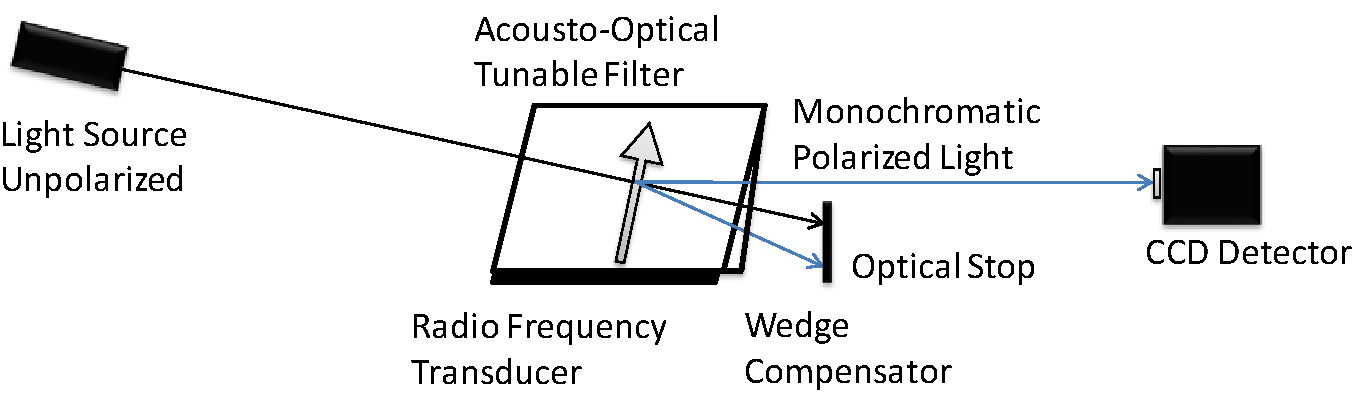
\includegraphics[width=1.0\textwidth]{./Images/3-1-AOTFGeneralLayout.pdf}
    \caption[Layout of an AOTF]{General Layout of an Acousto-Optical Tunable Filter. A randomly polarized incoming light source hits the front surface of the birefringent crystal. The black bar below the crystal is the piezo-electric transducer that produces the RF signal and forms the acousto wave represented by the grey arrow. The momentum matching Bragg diffraction occurs and monochromatic polarized light (+1 order) exits the the AOTF at a constant angle with the 0th order and -1 order being blocked by an optical stop.}
    \label{fig:3.1:AOTFLayout}
\end{figure}

In order for the AOTF to allow the filtering of a specific wavelength a momentum matching criteria must be held where the wave vectors of the acoustic wave match the difference of the incoming and diffracted light wave vectors. This condition is described by
\begin{equation}
    \ \mathbf{k}_{i} = \boldsymbol\kappa + \mathbf{k}_{d}
    \label{eqn:3.1:phaseMatching}
\end{equation}
where $\mathbf{k}_{i}$ and $\mathbf{k}_{d}$ are the wave vectors for the incoming and diffracted light and $\boldsymbol\kappa$ is the acoustic wave vector. These wave vectors can be described by
\begin{equation}
    \ k_{i} = \frac{2\pi n_{i}}{\lambda}
    \label{eqn:3.1:incomingWavevector}
\end{equation}
\begin{equation}
    \ k_{d} = \frac{2\pi n_{d}}{\lambda}
    \label{eqn:3.1:diffractedWavevector}
\end{equation}
\begin{equation}
    \ \kappa = \frac{2\pi F}{\nu}
    \label{eqn:3.1:acousticWavevector}
\end{equation}
where $n_{i}$ and $n_{d}$ are the indices of refraction of incoming and diffracted light. Finally $\lambda$ is the wavelength of light in a vacuum. It will be assumed that the extraordinary light is undergoes the momentum matching through the device. This causes the above refractive indices defined above to be
\begin{equation}
    \ n_{i} = \left( \frac{\sin^{2}(\theta_{i}+\alpha)}{n_{e}^{2}} + \frac{\cos^{2}(\theta_{i}+\alpha)}{n_{o}^{2}} \right)^{-\frac{1}{2}}
    \label{eqn:3.1:incomingIndexOfRefraction}
\end{equation}
\begin{equation}
    \ n_{d} = n_{o}
    \label{eqn:3.1:diffractedIndexOfRefraction}
\end{equation}
where $n_{e}$ and $n_{o}$ are the indices of refraction for the extraordinary and ordinary polarizations of the incoming light and $\alpha$ is the cut angle relative to the piezoelectric transducer and the optical axis. For a crystal, like TeO$_{2}$, the difference in the index of refraction is small and can be approximated as \citep{Voloshinov2007}
 \begin{equation}
    \ n_{i} = n_{o} + \Delta n\sin^{2}(\theta_{i}+\alpha)
    \label{eqn:3.1:incomingIndexOfRefractionApprox}
\end{equation}
where $\Delta n$ is the difference between the extraordinary and ordinary indices of refraction (ie $\Delta n = n_{e} - n_{o}$). The wave vectors, seen in \autoref{fig:3.1:ATOFWavevectors}, of the system need to follow the momentum matching criteria from \autoref{eqn:3.1:phaseMatching}. Separating the wave vectors into their directional components with respect to the cut angle, $\alpha$, the tangential and perpendicular directions respectively are
\begin{equation}
    \ k_{i}\cos\theta_{i} = {k}_{d}\cos\theta_{d}
    \label{eqn:3.1:wavevectorsTangentalDirection}
\end{equation}
\begin{equation}
    \ k_{i}\sin\theta_{i} + \kappa = {k}_{d}\sin\theta_{d}
    \label{eqn:3.1:wavevectorsPerepndicularDirection}
\end{equation}

\begin{figure}
    \begin{center}
    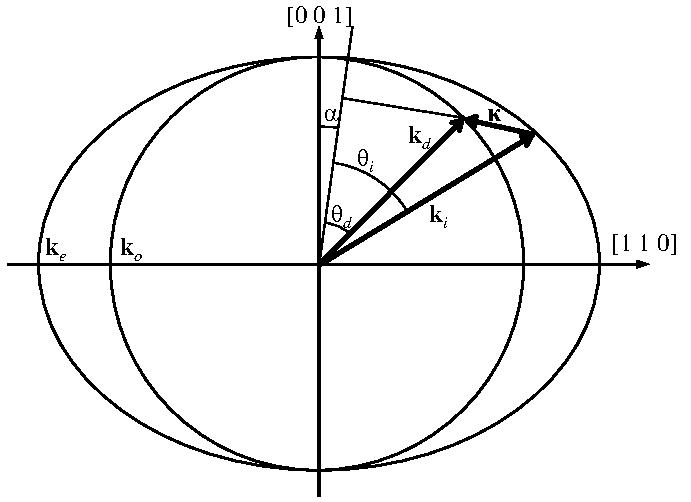
\includegraphics[width=0.7\textwidth]{./Images/3-1-AOTFWavevectorWithRefraction.pdf}
    \caption[Wave Vectors Generated by an AOTF]{The wave vectors generated by the AOTF experiment set up in \autoref{fig:3.1:AOTFExperimentalSetUp}. From the above figure $k_{e}$ and $k_{o}$ are the wave vectors of the extraordinary and ordinary axis of the AOTF crystal and can be represented as $2\pi n_{e}/\lambda$ and $2\pi n_{o}/\lambda$ respectively. The cut angel, $\alpha$, is the cut angle form the optional axis to the piezoelectric transducer.}
    \label{fig:3.1:ATOFWavevectors}
    \end{center}
\end{figure}

The tangential direction of the wave vector does not give any helpful information however the wavelength and RF relation can be determined by the perpendicular component of the wave vector by combining \autoref{eqn:3.1:wavevectorsPerepndicularDirection} and the vector diagram seen in \autoref{fig:3.1:ATOFWavevectors} to get
\begin{equation}
    \lambda  = \frac{\nu}{F}[n_{i}\sin\theta_{i}-(n_{o}^{2}-n_{i}^{2}\cos_{2}\theta_{i})^{1/2}]
    \label{eqn:3.1:initialAOTFWavelengthDependance}
\end{equation}

It should be noted that for the geometry defined the incident angle is the same as the Bragg angle. The above can be written as

\begin{equation}
    \lambda  = \frac{\Delta n\nu}{F}\frac{\sin^{2}(\theta_{i}+\alpha)}{\sin\theta_{i}}
    \label{eqn:3.1:AOTFWavelengthDependance}
\end{equation}
assuming difference in indices of refraction is small and the Taylor expansion approximation of the square root is used \citep{Voloshinov2006}. Also, through the described interaction the diffracted light goes though a 90\si{\degree} rotation in polarization \citep{Voloshinov1996}. Lastly, a wide aperture is required for an AOTF used for imaging purposes. These devices have been developed \citep{Gass1991} and are currently readily available for imaging purposes.

\subsection{Calibration and Testing}
\label{sec:3.1:AOTFCalibration}

In order to be able to preform the required spectral imaging a large aperture imaging quality ATOF was acquired from Brimrose of America. It is optically tuned for a range of 600 nm to 1200 nm and made from a Tellurium Dioxide (TeO$_{2}$) birefringent crystal. The extraordinary light is diffracted at 2.7\si{\degree} off of the optical axis of the device. In order to achieve a constant diffraction angle of the first order beam a wedge is attached to the exit aperture of the AOTF to compensate for the angular change that occurs from altering the filtered wavelength.  The device has a fast RF stabilization time and the diffraction efficiency can be varied by changing the RF power. A set of characterizations experiments were performed on this crystal.

A test optical set up was devised in the lab to determine the RF and output wavelength relation, the Full Width Half Max (FWHM), and transmission of the Brimrose AOTF. A telecentric test layout was used, which will be described in \autoref{sec:3.2:telecentricSystem}. An advantage of the telecentric design is that the wavelength dependance of the acousto effect from the incident angle is removed since all the lines of sight enter the AOTF at the same angular spread. The AOTF was located in the center of two 100~mm focal length lenses. An aperture was set up in front and behind the AOTF optical chain at the focal length of the front and back lenses respectively and opened to 5~mm. The high front end f-number of 20 required long integration times for capture but the light entering the spectrometer optics were well collimated and limited the amount of stray light. It also enabled the system to have a much higher degree of telecentricity. A polarizer was inserted on either side of the AOTF to remove the ordinary polarized light on the entrance side and the 0th order light on the exit side of the device. Also two prisms were used to compensate for the 2.7\si{\degree} off axis bending to set the light back on the the optical path just offset slightly from the optical axis but traveling parallel to it. A standard 20~W tungsten halogen bulb was used as a light source. The front end optics had no magnification and back optics were used to match the f-number of the spectrometer's input optics. The layout can be seen in \autoref{fig:3.1:testExperimentalSetup}.

\begin{figure}
    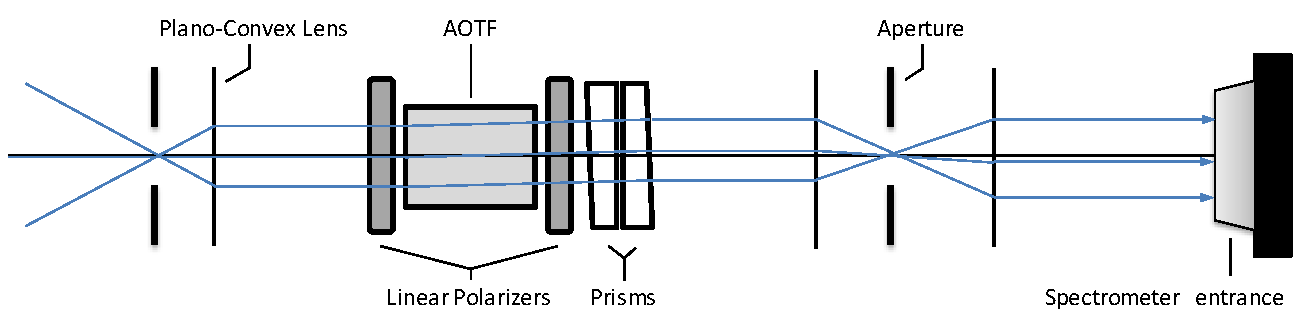
\includegraphics[width=1.0\textwidth]{./Images/3-1-TestExperimentalSetUp.pdf}
    \caption[AOTF Calibration Experimental Setup]{Telecentric test experiential setup for AOTF parameter determination. All lenses and apertures are represented by the same symbol.}
    \label{fig:3.1:testExperimentalSetup}
\end{figure}

%not in orginal
%\begin{figure}[h]
%    \begin{minipage}{.5\textwidth}
%    \includegraphics[width=0.97\textwidth]{./Images/gratingTransmission.png}
%    \end{minipage}
%    \begin{minipage}{.5\textwidth}
%    \includegraphics[width=0.97\textwidth]{./Images/SynCcdTransmission.png}
%    \end{minipage}
%    \caption{Left: The transmission characteristics for the 1200 lines per millimeter grating used in the iHR320 spectrometer. Right: The transmission characteristics for the Synpase CCD. Both transmission characteristics curtsey of HORIBA.}
%    \label{fig:HoribaTransmission}
%\end{figure}

The spectrometer is a HORIBA iHR320 with a 1200~lines/mm grating blazed at 750~nm. The CCD attached to the spectrometer is a Synopse CCD detector, model number SYN-1024x256-OE. It is thermoelectricity cooled to -75\si{\degree\celsius} to reduce any significant dark current contributions to the measurements.

Images were taken at a set of RFs spaced every 150 kHz from 160~MHz to 75~MHz and the spectral images were recorded with the spectrometer slit at 0.5~mm making the minimum FWHM of the spectrometer 1.175~nm, which is well below the minimum FWHM of the AOTF listed specifications at 1.6~nm. For each trial at each RF two images were taken with a 15~second integration time: one taken with the AOTF on at a given RF and one with the ATOF off. The stray light entering spectrometer as well as the any dark current and the DC bias are recorded in the image with the AOTF off and can be removed from the AOTF spectral image by taking the image with the AOTF on and subtracting the image recorded with the AOTF off. Then all of the rows of the CCD are summed together to get the total count measurement at each wavelength. The maximum value of each image is taken to be the diffracted wavelength through the AOTF at each respective RF. A typical spectral measurement result can be seen in the top left panel of \autoref{fig:3.1:AOTFCharaterization}. The characteristic sinc function filtering can be seen in the image. Typically the fringes of the sinc function accounts for 16\% of the total signal.

\begin{figure}
    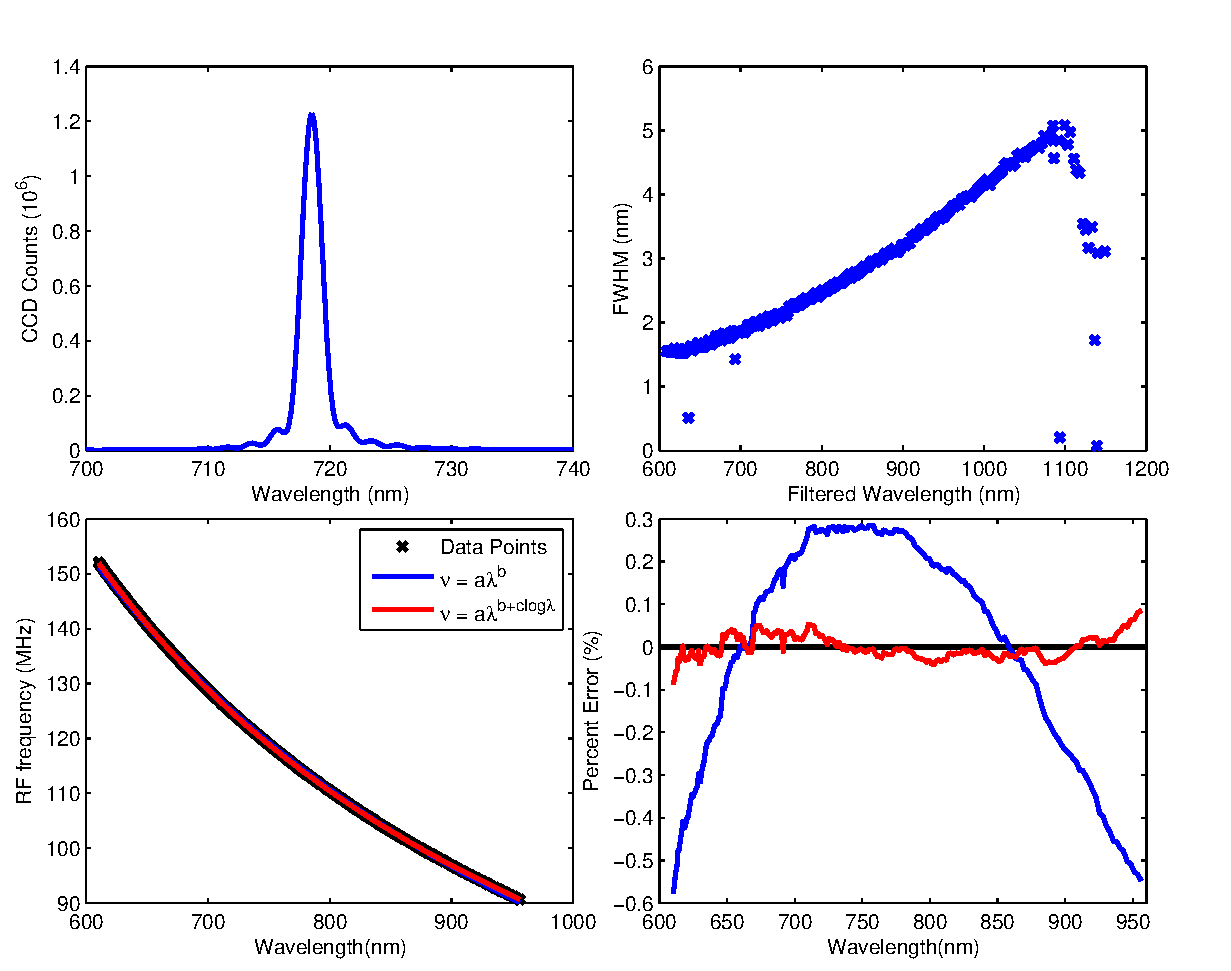
\includegraphics[width=1.0\textwidth]{./Images/3-1-AOTFCharaterization.pdf}
    \caption[Characterization Curves for the Brimrose AOTF]{Top Left: A standard image taken from the AOTF calibration experiment when the tuning frequency of the AOTF was at 124.96~MHz. Top Right: The FWHM for each of the determined wavelengths for the AOTF. It should be noted that the FWHM at 600~nm is 1.5~and as the wavelengths get longer the FWHM increases to 4.9 at 1080~nm. Bottom Left: The calibration curves for the AOTF RF versus the  diffracted wavelength which contains the data points recorded and two best fit curves. Bottom Right: The percent error with respect to the measured frequency for the two best fit curves in the previous panel. It can be noted the modified power function approximates the AOTF wavelength dependance to within 0.1\%.}
    \label{fig:3.1:AOTFCharaterization}
\end{figure}

The maximum values from each of the images were determined as well as the wavelength these values occur. It was noted that the curve appear to follow a power function of the form
\begin{equation}
    \ F = a\lambda^{b}.
    \label{eqn:3.1:powerFunction}
\end{equation}
A linear least squares fit was preformed in log space finding the coefficients $a$ and $b$. The fit was performed and appeared to match the data quite well but a relative error analysis was preformed and it was seen that there was a only an agreement better than 0.6\%. A better fit was desired to characterize the AOTF's RF-spectral dependance so a modified power function was used in the form of
 \begin{equation}
    \ F = a\lambda^{b+c\log\lambda}
    \label{eqn:3.1:modifiedPowerFunction}
\end{equation}
or a quadratic least squares fit. These results can be seen in the bottom half of \autoref{fig:3.1:AOTFCharaterization}. The agreement of this form is less than 0.1\% throughout the whole wavelength range and the determined RF and wavelength relation can be seen in
\begin{equation}
    \ F = \exp{19.793}\lambda^{-3.381+0.168\log\lambda}.
    \label{eqn:3.1:modifiedPowerFunctionCoeffiecicents}
\end{equation}
It should be noted that even though the AOTF optical range is 600~nm to 1200~nm this analysis only measures wavelengths from 600~nm to 950~nm. The low quantum efficiency of the CCD and the low NIR emitted from the light source causes wavelengths past this point to be noisy. Thus these measurements were left out and an InGaAs array with better quantum efficiency in the NIR has been acquired and will be used to characterize the rest of the spectral range of the AOTF.

The same set of data was used to determine the FWHM for each of the above determined wavelengths. the results of this study are shown in the top right of \autoref{fig:3.1:AOTFCharaterization}. Wavelengths past approximately 1080~nm are to noisy too be able to determine the FWHM of the signal and will be determined at a later date with the InGaAs Array. However, the AOTF spectral resolution is well within the limits that are required in order to determine aerosol extinction and cloud occurrence in the UTLS.

The diffraction efficiency was also determined for a few points across the wavelength range of the AOTF and the wavelengths results were all within 56$\%$ to 64$\%$ as were stated by the factory specification of the device. Two limb imaging systems have been prototyped for use with the AOTF and their characteristics including advantages and problems will discussed in the following sections. 